\documentclass[a4paper, 11pt]{article}
\usepackage[UTF8]{ctex}
\usepackage{amsmath}
\usepackage{graphicx}
\usepackage{geometry}
\usepackage{listings}
\geometry{scale=0.8}
\usepackage{hyperref}
\linespread{1.5}

\title{	
\normalfont \normalsize
\textsc{School of Data and Computer Science, Sun Yat-sen University} \\ [25pt] %textsc small capital letters
\rule{\textwidth}{0.5pt} \\[0.4cm] % Thin top horizontal rule
\huge  T01 Search and game tree search\\ % The assignment title
\rule{\textwidth}{2pt} \\[0.5cm] % Thick bottom horizontal rule
\author{16337110 匡乾, 16337111 赖若潘}
\date{\normalsize\today}
}

\begin{document}
\maketitle
\tableofcontents
\newpage
\section{Q1}
\begin{figure}
  \centering
  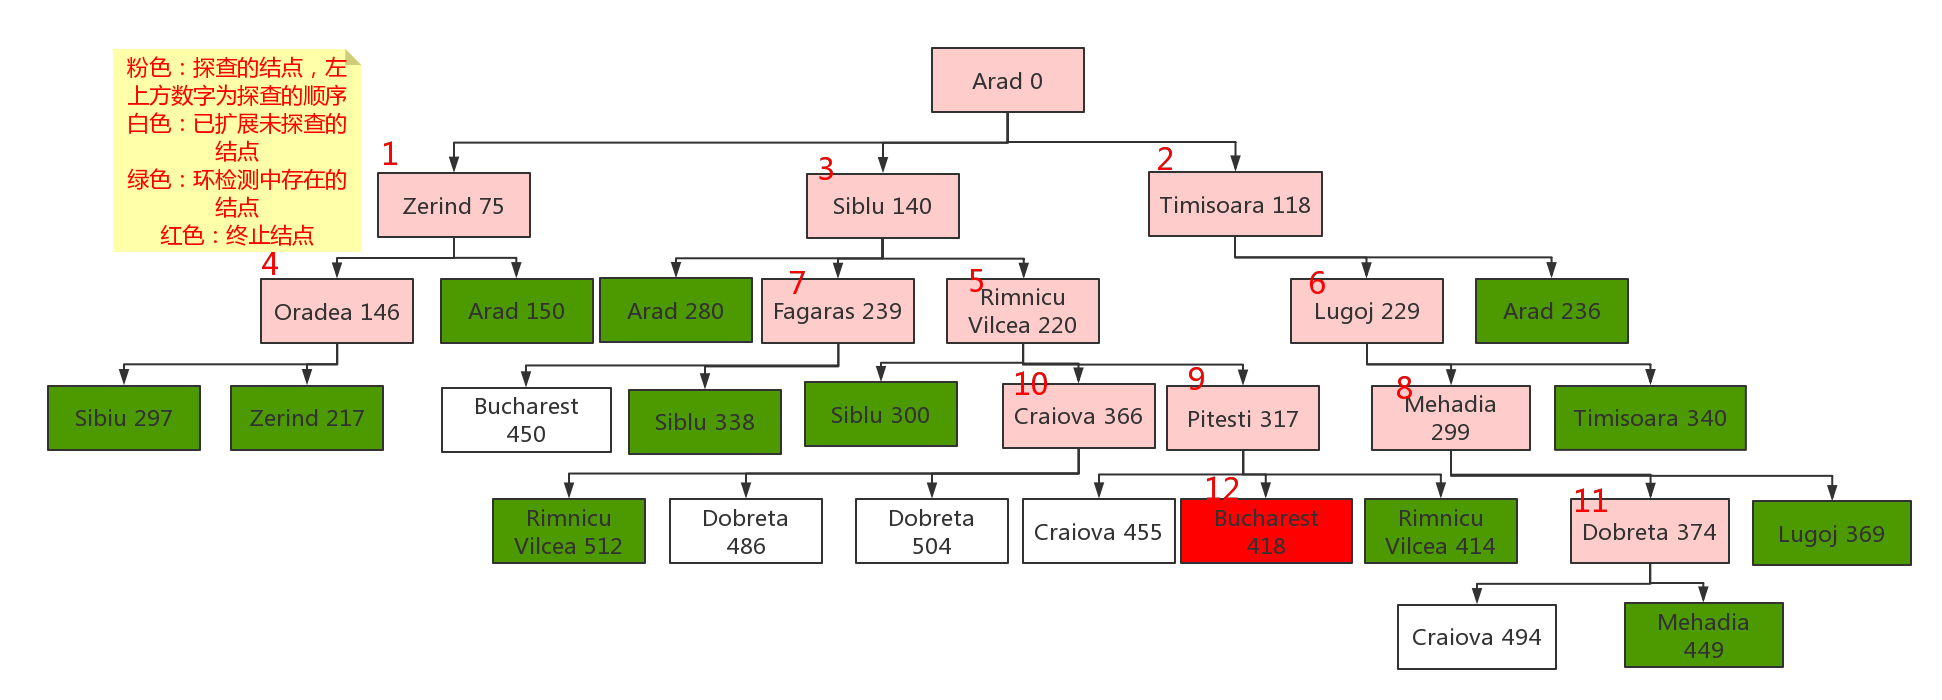
\includegraphics[width=15cm]{0.png}
  \caption{Q1 search tree}
\end{figure}

Frontier

0. \{Arad 0\}

1. \{Zerind 75, Timisoara 118, Sibiu 140\}

2. \{Timisoara 118, Sibiu 140, Oradea 146\}

3. \{Sibiu 140, Oradea 146, Lugoj 229\}

4. \{Oradea 146, Rimnicu Vilcea 220, Lugoj 229, Fagaras 239\}

5. \{Rimnicu Vilcea 220, Lugoj 229, Fagaras 239, (Sibiu 297)\}

6. \{Lugoj 229, Fagaras 239, Pitesti 317, Craiova 366\}

7. \{Fagaras 239, Mehadia 299, Pitesti 317, Craiova 366\}

8. \{Mehadia 299, Pitesti 317, Craiova 366, Bucharest 450\}

9. \{Pitesti 317, Craiova 366, Dobreta 379, Bucharest 450\}

10. \{Craiova 366, Dobreta 379, Bucharest 418, Bucharest 450, Craiova 455\}

11. \{Dobreta 379, Bucharest 418, Bucharest 450, (Craiova 455), Dobreta 486, (Pitesti 504)\}

12. \{Bucharest 418, Bucharest 450, (Dobreta 486), (Craiova)\}

13. [terminal] Bucharest 418

\section{Q2}


	先证明一致性,可直接推得可采纳性

	首先先证明:$h1(n) \in \{0,1,2,3\}$, $h2(n) \in \{0,1,2\}$。

	h1(n)显然,现证明h2(n),$h2(n)>0$的所有情况如图所示

    \begin{figure}
      \centering
      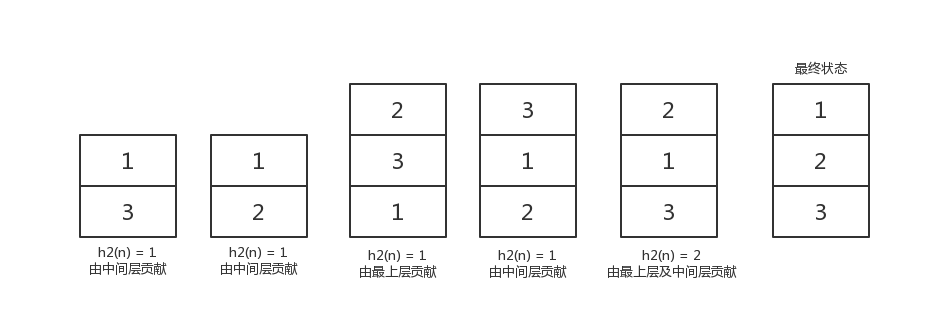
\includegraphics[width=15cm]{5.png}
      \caption{$h2(n)>0$的所有情况}
    \end{figure}

	综上,$h2(n) \in \{0,1,2\}$,且显然每一个砖块最多给h2(n)贡献1。

	要证明一致性,即证明$h(n1) \le c(n1,n2) + h(n2)$,即证明$\Delta h(n) \le 1$ $(\Delta h(n)=h(n1)-h(n2))$,证明如下:

	因为每一次挪动只改变一个砖块的位置,故$\Delta h1(n) = 0 \ or \pm1$,而由$h2(n)>0$的所有情况图来看,每一层(砖块)最多贡献1,即h2(n)不可能由0变为2或是2变为0,故$\Delta h2(n) = 0 \ or \pm1$。


	现证明:$\Delta h(n) =  \Delta h1(n)+\Delta h2(n) \le 1$
	\begin{enumerate}
	\item 当$\Delta h1(n) = 0 \ or -1$时,直接成立
	\item 当$\Delta h1(n) = 1$时,此时可能有三种操作,分类进行讨论:
		\begin{enumerate}
		\item 从高处拿下一个砖块放到地板上,即这一块砖在goal state中为底层砖,故移动其不影响h2(n),这种情况下$\Delta h2(n) = 0$,故成立
		\item 从高处拿下一个砖块放到另一块砖上面,这种情况在$\Delta h1(n) = 1$时不可能出现,因为该砖在只有三块砖的体系中,这种移动并没有改变这块砖的高度位置
		\item 从地板上拿起一块砖放到另一块砖上面,原先这块砖下面没有砖块,且此时这块砖处于goal state,故$\Delta h2(n) = 0$
		\end{enumerate}
		综上,当$\Delta h1(n) = 1$时,$\Delta h2(n) = 0$
	\end{enumerate}

	故综上,$\Delta h(n) =  \Delta h1(n)+\Delta h2(n) \le 1$成立。

	一致性得证,则可采纳性也可以得到。

	故h是可采纳的,一致的。

    \newpage

    \begin{figure}
      \centering
      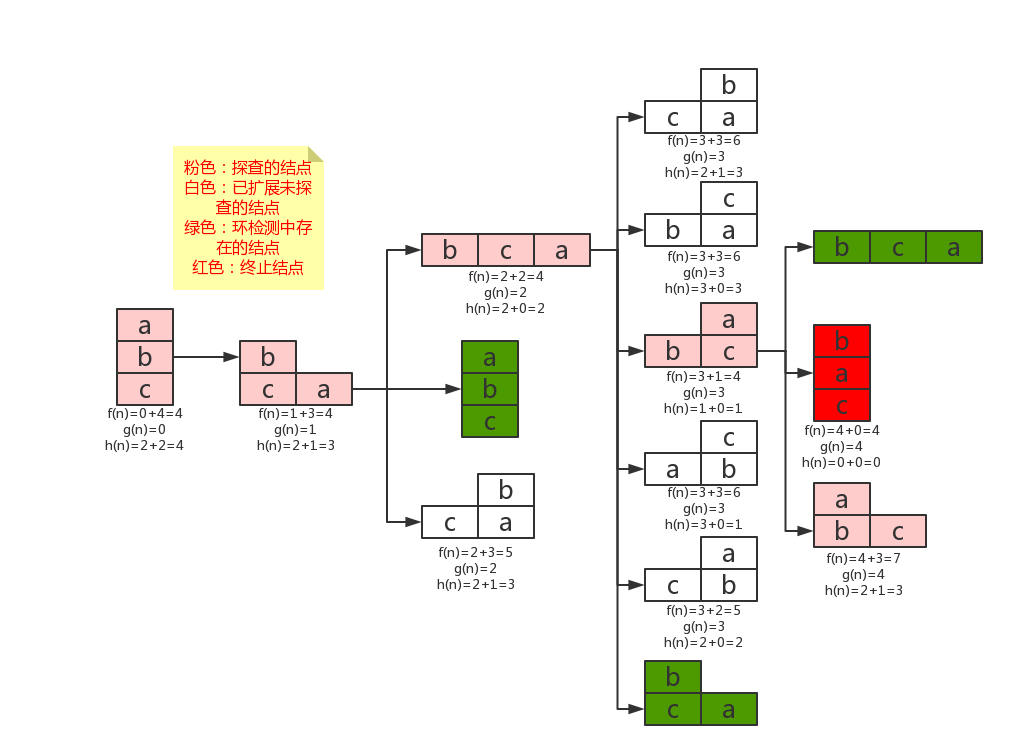
\includegraphics[width=15cm]{4.png}
      \caption{A* search tree}
    \end{figure}


\section{Q3}
\begin{figure}
  \centering
  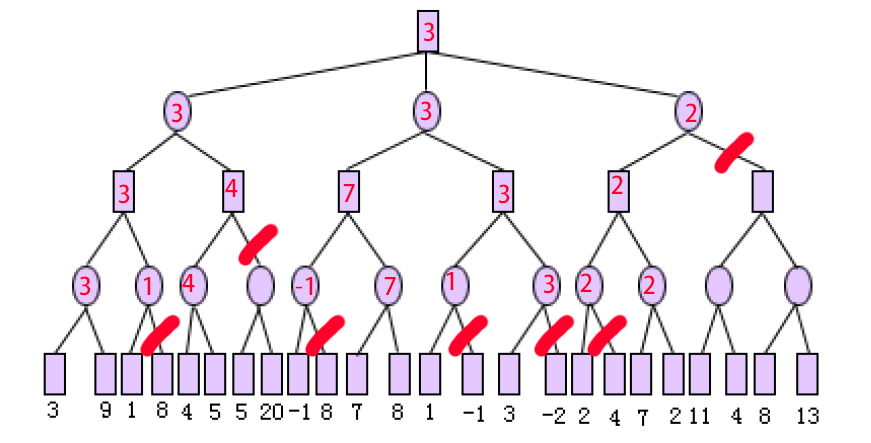
\includegraphics[width=15cm]{3.jpg}
  \caption{$\alpha-\beta$ pruning}
\end{figure}

%\clearpage
%\bibliography{E:/Papers/LiuLab}
%\bibliographystyle{apalike}
\end{document}


%%% Local Variables:
%%% mode: latex
%%% TeX-master: t
%%% End:
